\documentclass[./PianoDiProgetto.tex]{subfiles}
\begin{document}
\section{Pianificazione}
  Elenchiamo qui di seguito le caratteristiche e le durate di ogni periodo. Nella decisione dei tempi sono stati tenuti in considerazione e si sono cercati di mitigare i rischi relativi alle tempistiche.
	\subsection{\PerAR{} (AR)}
  \textbf{Periodo: dal 2016-12-10 al 2017-01-11}

  Questo periodo comincia con il primo incontro del gruppo e termina con la scadenza della consegna riguardante la \textbf{Revisione dei requisiti}.

  È composto principalmente dalle seguenti attività:
  \begin{enumerate}
		\item \textbf{scelta degli strumeti}: verranno scelti gli strumenti che saranno utilizzati per la stesura dei documenti e per il supporto. La scelta degli strumenti sarà ?incrementale? nel corso del progetto;
		\item \textbf{stesura delle Norme di progetto}: dopo aver scelto i primi strumenti per la produzione di documentazione sarà possibile iniziare la stesura delle \NPdocRR. Questo documento sarà utilizzato indipendentemente dal capitolato che verrà preso in appalto, e sarà steso in modo incrementale via via che nuove norme verrano definite;
		\item \textbf{stesura documentazione}: una volta definiti norme e strumenti per la scrittura di un documento, è possibile iniziare la stesura dei seguanti documenti;
    \begin{itemize}
      \item Analisi dei Requisiti: si redige il documento \ARdocRR. Verrano organizzati degli incontri col proponente, sia prima che durante la stesura di questo documento, per consolidare i requisiti stesi e per chiarire eventuali dubbi sui requisiti da stendere;
      \item Studio di fattibilità: vengono valutati pro e contro di tutti i capitolati proposti e viene redatto il documento \SFdocRR. Viene quindi scelto il capitolato da sviluppare;
      \item Piano di Progetto: viene steso il documento \PPdocRR, il quale regolerà le attività le attività del gruppo;
      \item Piano di qualifica: si stende il documento \PQdocRR per fissare quali sono gli standard di qualità ed in che modo il gruppo si prefigge di raggiungerli;
      \item Glossario: viene creato il file incrementale "terminiGlossario.txt" e steso in modo automatico il documento \GldocRR.
      \item Lettera di Presentazione: si scrive la lettera in cui si dichiara l'interesse del gruppo a partecipare alla gara di appalto.
      \item Analisi preliminare degli SDK dei principali assistenti virtuali: gli \ANP{} analizzeranno gli SDK dei principali assistenti virtuali, dotati di intelligenza artificiale, presenti sul mercato, e scriveranno il documento esterno \textit{AnalisiSDK v1.0.0} in cui verrà effettuato il confronto tra  essi.
    \end{itemize}
  \end{enumerate}
  %\newpage
  \subsubsection{Diagramma di Gantt - \PerAR}
    \begin{figure}[!h]
    \centering
    %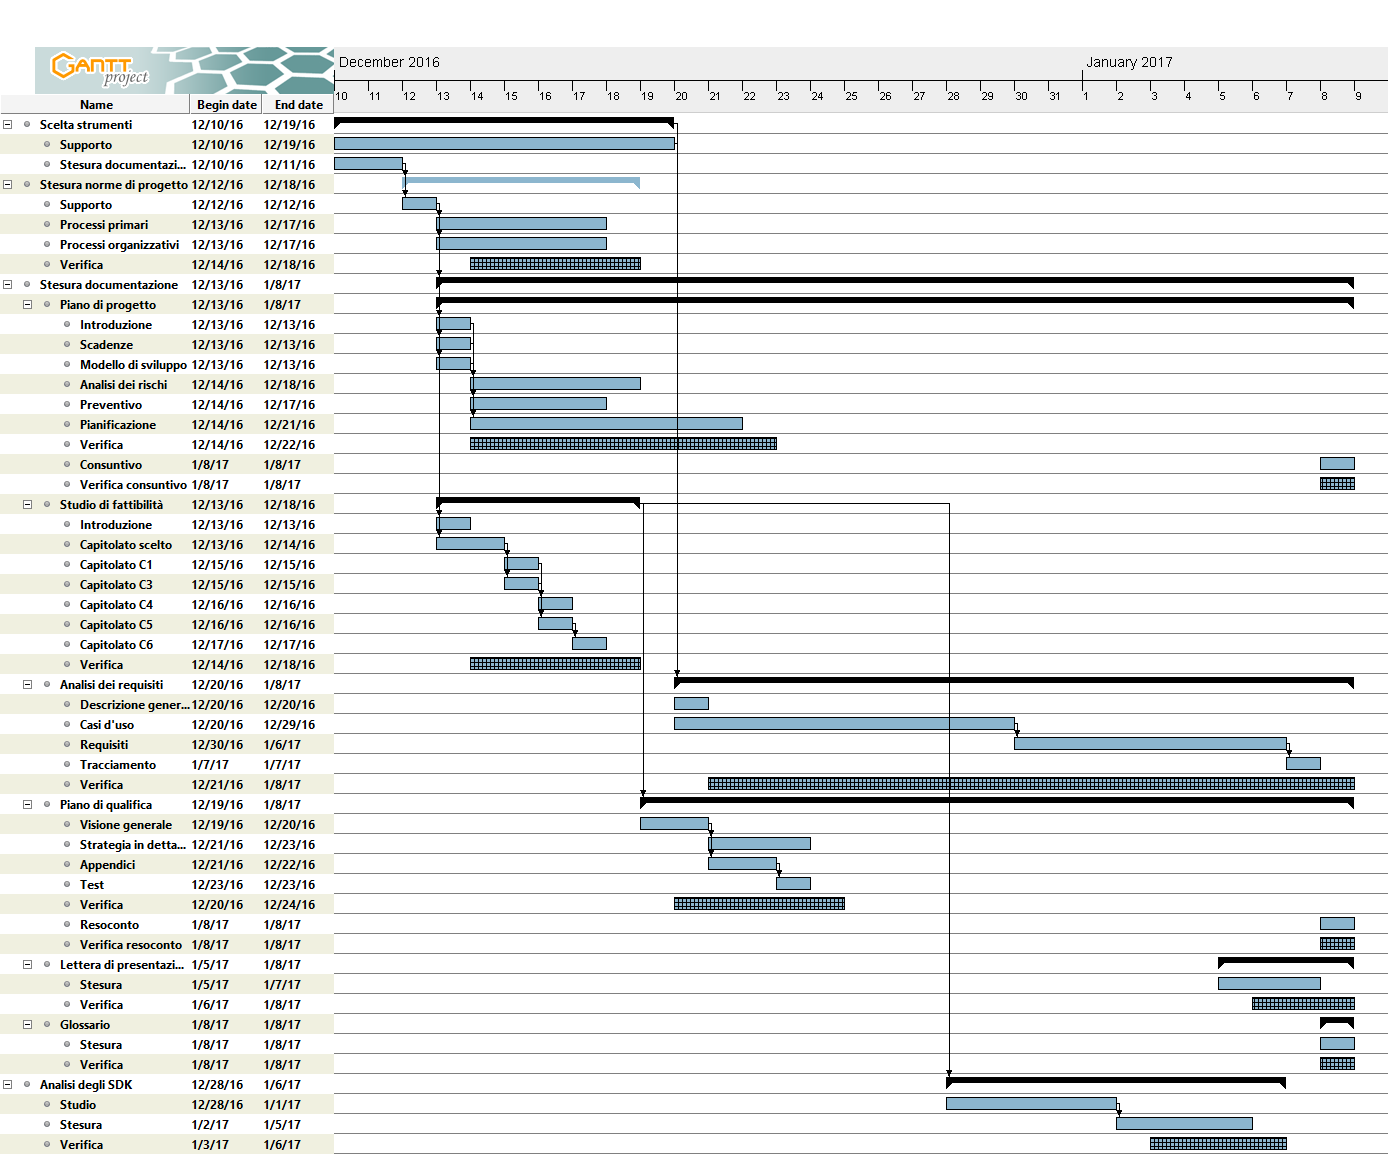
\includegraphics[width=\textwidth]{images/AR}
    \caption{Gantt - \PerAR}
    \end{figure}

	\subsection{\PerAD{} (AD)}
  \textbf{Periodo: dal 2016-01-12 al 2016-02-22}

  %\newpage
  \subsubsection{Diagramma di Gantt - \PerAD}
    \begin{figure}[!h]
    \centering
    %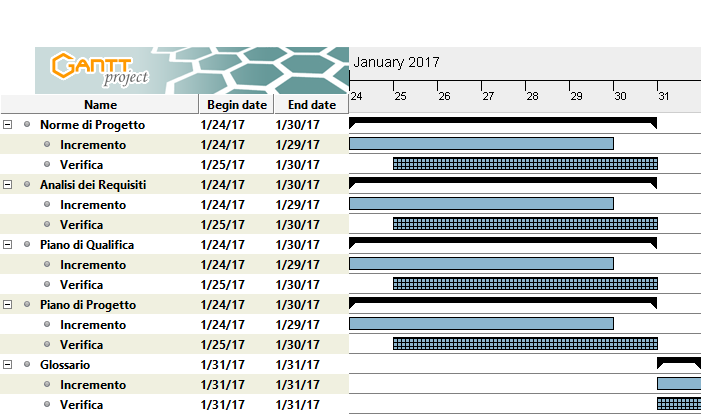
\includegraphics[width=\textwidth]{images/AD}
    \caption{Gantt - \PerAD}
    \end{figure}

  \subsection{\PerPA{} (PA)}
  \textbf{Periodo: dal 2016-02-23 al 2016-03-14}

  Questo periodo comincia al termine del periodo A. Tutti i documenti prodotti nel periodo precedente vengono incrementati e corretti in base alle segnalazioni del committente e del proponente. Gli analisti provvedono ad individuare nuovi requisiti e a correggere eventuali requisiti segnalati; in seguito si provvede all'incremento di tutti gli altri documenti. In seguito all'aggiornamento dei requisiti, verrà organizzato un incontro col proponente per la loro verifica.
  %\newpage
  \subsubsection{Diagramma di Gantt - \PerPA}
    \begin{figure}[!h]
    \centering
    %\includegraphics[width=\textwidth]{images/PDR}
    \caption{Gantt - \PerPA}
    \end{figure}

  \subsection{\PerPDR[]{} (PDR)}

  Questo periodo inizia con la fine del periodo PA. È stato suddiviso in tre sottoperiodi, per differenziare tra i requisiti di diversa priorità.

  \subsubsection{\PerPDROB{} (PDROB)}
  \textbf{Periodo: dal 2016-01-12 al 2016-02-22}

  È il primo dei sottoperiodi. Il suo inizio coincide con l'inizio della \PerPDR[], e la sua fine coincide con la consegna della \textbf{Revisione di Progettazione}. Le attività svolte durante questo consistono in:
  \begin{itemize}
    \item Definizione di prodotto: viene steso il documento \textit{Definizione di Prodotto v1.0.0}. Esso definisce la struttura interna del sistema e le relazioni tra i diversi moduli del prodotto, per quanto riguarda i requisiti obbligatori;
    \item codifica: inizia lo sviluppo da parte dei programmatori dei moduli del sistema atti a soddisfare i requisiti obbligatori. Sarà guidato da quanto riportato nel documento \textit{Definizione di Prodotto v1.0.0};
    \item incremento e verifica dei documenti: se ritenuto necessario vengo apportate modifiche ai documenti già stilati;
    \item Glossario: vengono aggiunti al \textit{Glossario} i vocabili dei quali si ritenga necessaria una definizione formale.
  \end{itemize}

  %\newpage
  \paragraph{Diagramma di Gantt - \PerPDROB}
    \begin{figure}[!h]
    \centering
    %\includegraphics[width=\textwidth]{images/PDROB}
    \caption{Gantt - \PerPDROB}
    \end{figure}

  \subsubsection{\PerPDRD{} (PDRD)}
  \textbf{Periodo: dal 2016-01-12 al 2016-02-22}

  Questo sottoperiodo inizia in seguito all'esito della \textbf{Revisione di Progetto}. Le attività di questa fase saranno le seguenti

  %\newpage
  \paragraph{Diagramma di Gantt - \PerPDRD}
    \begin{figure}[!h]
    \centering
    %\includegraphics[width=\textwidth]{images/PDRD}
    \caption{Gantt - \PerPDRD}
    \end{figure}

  \subsubsection{\PerPDROP{} (PDROP)}
  \textbf{Periodo: dal 2016-01-12 al 2016-02-22}

  %\newpage
  \paragraph{Diagramma di Gantt - \PerPDROP}
    \begin{figure}[!h]
    \centering
    %\includegraphics[width=\textwidth]{images/PDROP}
    \caption{Gantt - \PerPDROP}
    \end{figure}

  \subsection{\PerV (V)}
  \textbf{Periodo: dal 2016-01-12 al 2016-02-22}

  %\newpage
  \subsubsection{Diagramma di Gantt - \PerV}
    \begin{figure}[!h]
    \centering
    %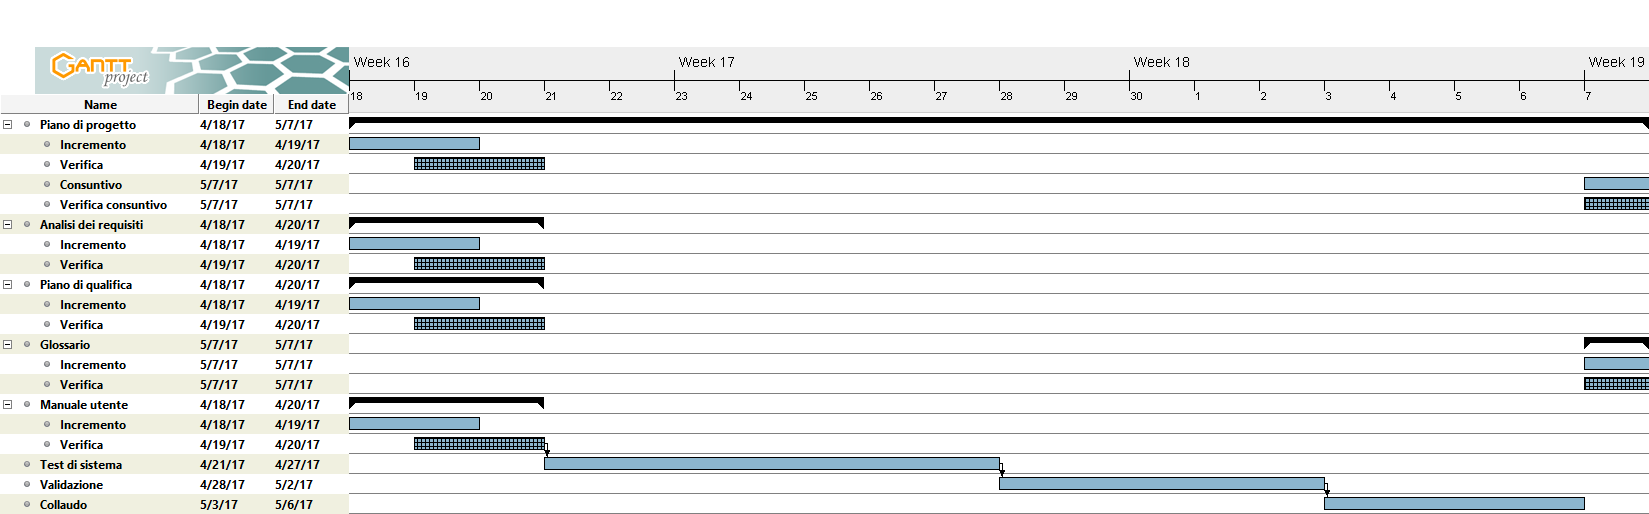
\includegraphics[width=\textwidth]{images/V}
    \caption{Gantt - \PerV}
    \end{figure}
\end{document}
